% !TEX root = ../documentation.tex

\chapter{Testing}
In diesem Kapitel werden verschiedene Konzepte vorgestellt, die zum Testen der Applikation angewandt werden sollen.

\section{Black-Box-Tests}
Die Verwendung des Black Box Tests dient zur Überprüfung der Spezifikationen und des Prozessablaufes.
Zur Erkennung von Softwarefehlern soll ein inkorrektes Systemverhalten ausgelöst werden, indem z.B. unerwartete oder falsche Eingaben durchgeführt werden.
Dieses Vorgehen soll exemplarisch an dem Anmelde- und Registrierungsprozess konzipiert werden.

Betrachten wir den Registrierungsprozess, bei dem der Nutzer dazu angehalten ist, einen Benutzernamen, eine Email-Adresse, ein Passwort und eine Telefonnummer anzugeben. 
Sowohl bei der Wahl des Benutzernamens, als auch des Passworts sind zugrundeliegende Richtlinien einzuhalten. Zusätzlich wird überprüft, ob die Email-Adresse der Syntax \emph{local\_part}@\emph{host\_name.top\_level\_domain} folgt und die Telefonnummer aus maximal 15 Ziffern besteht. Um eine Registrierung abschließen zu können, muss der Nutzer außerdem die Datenschutzbestimmungen akzeptieren und seine Eingabe bestätigen.
Werden diese Regeln eingehalten, so kann sich der Nutzer problemlos registrieren, vorausgesetzt der Benutzername und/oder Email-Adresse sind noch nicht registriert.
Im Falle des Anmeldeprozesses muss überprüft werden, ob die Eingabe der Anmeldedaten ohne Probleme möglich ist, und ob das Verhalten bei Betätigung der Anmeldeschaltfläche nach den Vorgaben abläuft.
Bei diesem Prozess werden lediglich Email-Adresse und Passwort erfragt und überprüft, ob ein Nutzer mit dieser Email-Adresse vorhanden ist und das eingegebe Passwort korrekt ist. 
Um die Anwendung auf Softwarefehler zu untersuchen, werden zunächst Testfälle entworfen und die dazugehörigen Testdaten erstellt. Anschließend wird die Anwendung mit den erstellten Testdaten ausgefüht und ein Testprotokoll erstellt. 

\begin{figure}
\centering
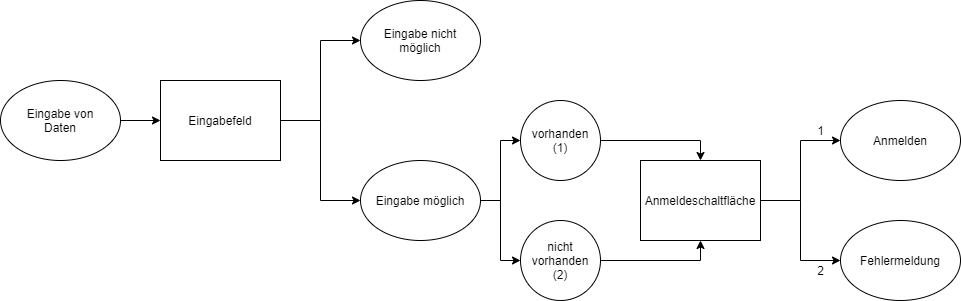
\includegraphics[width=\textwidth]{images/text/bbtest.png}
\label{fig:blackbox}
\caption{Black-Box-Test Prozessablauf}
\end{figure}


Im Folgenden werden denkbare Testfälle und dazugehörige Testdaten vorgestellt.

\begin{table}
\centering
\begin{tabular}{p{4.5cm}|p{4.5cm}|p{4.5cm}}
Testfall									& Testdaten												& Erwartete Ergebnis\\
\hline
Feld Benutzername leer						& \emph{keine Eingabe}									& Fehlermeldung Benutzername fehlt\\
Benutzername bereits vergeben				& Bereits registrierter Benutzernamen 					& Fehlermeldung Nutzer bereits vorhanden\\
Benutzername erfüllt Anforderungen nicht	& 														& Fehlermeldung Benutzername ungültig\\
Benutzername erfüllt Anforderungen			&														& Registrierung möglich\\
Feld Passwort leer							& \emph{keine Eingabe}									& Fehlermeldung Passwort fehlt\\
Passwort erfüllt Anforderungen nicht		& 														& Fehlermeldung Passwort zu unsicher\\
Passwort erfüllt Anforderungen				& Test1234!												& Registrierung möglich\\
Feld Email leer								& \emph{keine Eingabe}									& Fehlermeldung Email fehlt\\
Email-Syntax nicht eingehalten				& test.de 												& Fehlermeldung Email ungültig\\
Email-Syntax eingehalten					& test@test.de 											& Registrierung möglich\\
Email bereits registriert 					& \emph{bereits registrierte Email}						& Fehlermeldung Nutzer bereits vorhanden\\
Feld Telefon leer 							& \emph{keine Eingabe}									& Fehlermeldung Telefon fehlt\\
Telefonnummer erfüllt Anforderungen nicht	& 1234567890123456										& Fehlermeldung Telefonnummer ungültig\\
Telefonnummer erfüllt Anforderungen			& 123456789012345										& Registrierung möglich\\
Datenschutzbestimmungen nicht akzeptiert	& \emph{Checkbox nicht aktiviert}						& Fehlermeldung Datenschutzbestimmungen müssen akzeptiert werden\\
Datenschutzbestimmungen akzeptiert			& \emph{Checkbox aktiviert}								& Registrierung möglich\\

\end{tabular}
\label{tab:testing:fehlertest:registrierung}
\caption{Konzept Fehlertests - Testfälle und Testdaten Registrierungsprozess}
\end{table}

\begin{table}
\centering
\begin{tabular}{p{4.5cm}|p{4.5cm}|p{4.5cm}}
Testfall									& Testdaten												& Erwartete Ergebnis\\
\hline
Feld Email leer								& \emph{keine Eingabe}									& Fehlermeldung Anmeldung fehlgeschlagen\\
Email nicht registriert 					& \emph{nicht registrierte Email} 						& Fehlermeldung Nutzer nicht bekannt\\
Feld Passwort leer							& \emph{keine Eingabe}									& Fehlermeldung Anmeldung fehlgeschlagen\\
Passwort falsch 							& \emph{falsches Passwort} 								& Fehlermeldung Passwort falsch\\
Email und Passwort korrekt					& \emph{korrekte Zugangsdaten} 							& Anmeldung möglich\\

\end{tabular}
\label{tab:testing:fehlertest:anmeldung}
\caption{Konzept Fehlertests - Testfälle und Testdaten Anmeldeprozess}
\end{table}

\clearpage
\section{Strukturelle Tests}
Als Strukturellen Test bezeichnet man die Code Analyse, die dazu dient, anhand des Codes alle erforderlichen Testfälle herauszufinden, die benötigt werden, um jede Anweisung im Verlauf des Testprogramms einmal auszuführen.
Der Pfadüberdeckungstest ist eine Strategie des Strukturellen Tests. Hier besteht das Ziel darin, alle unabhängigen Pfade ausfindig zu machen, damit beim Testen jeder Pfad und somit auch jede Anweisung darin ausgeführt werden kann.

Bei der Gruppenerstellung sieht der Kontrollflussgraph mit allen Schleifen und Verzweigungen folgendermaßen aus:

\begin{figure}[!h]
\centering
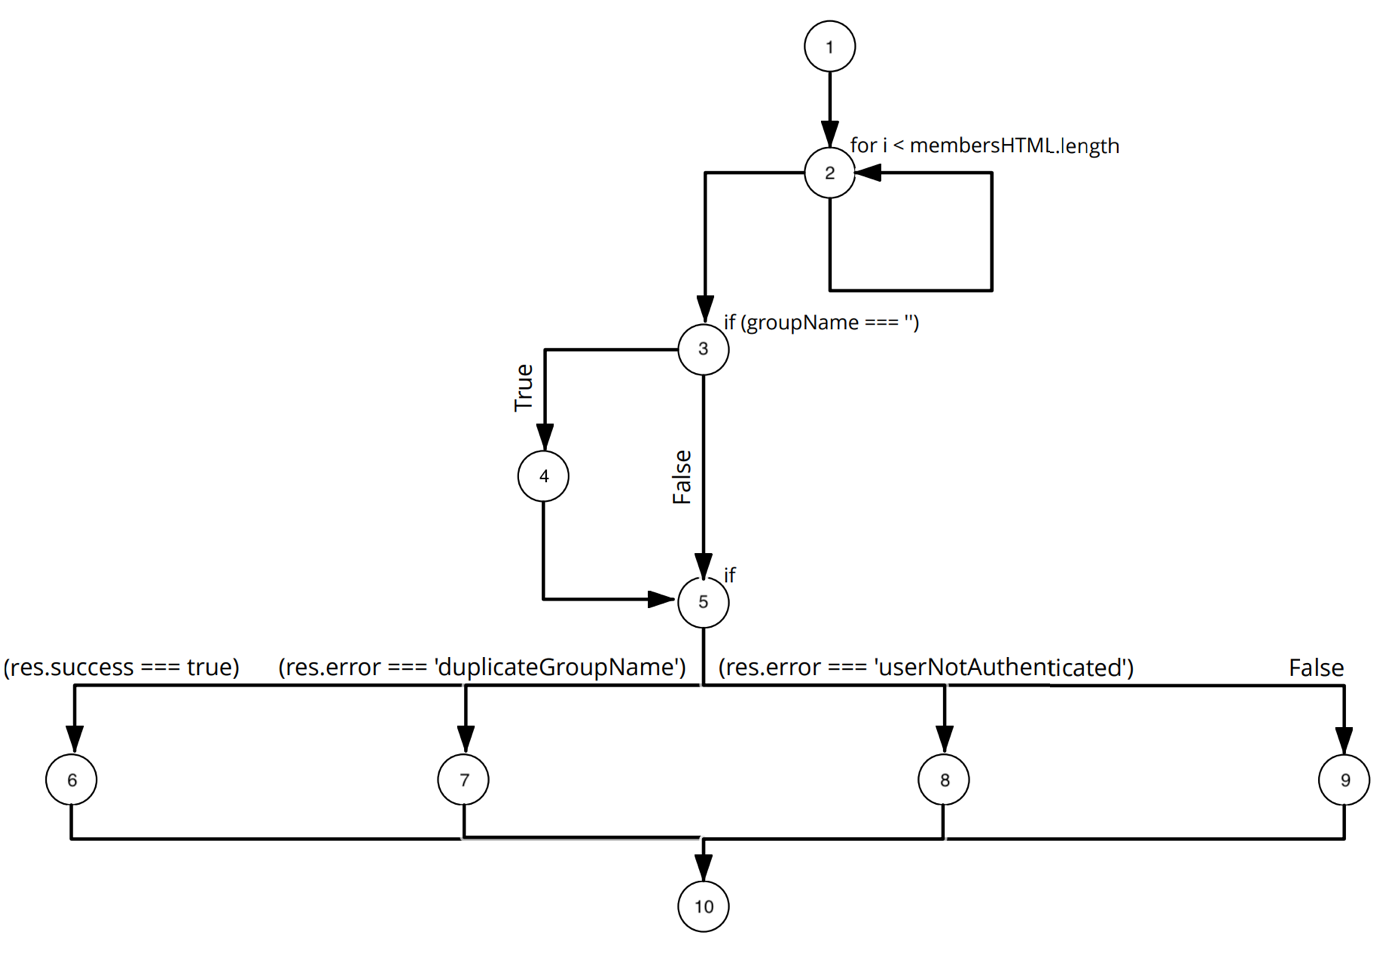
\includegraphics[width=\textwidth]{images/text/strukturelle_tests.png}
\label{fig:strukturelle_tests}
\caption{Kontrollflussgraph für Gruppenerstellungsprozess}
\end{figure}

Hieraus lassen sich folgende unabhängige Pfade herleiten:
\begin{itemize}{}{}
\item 1,2(beliebig oft),3,4,5,6,10
\item 1,2(beliebig oft),3,4,5,7,10
\item 1,2(beliebig oft),3,4,5,8,10
\item 1,2(beliebig oft),3,4,5,9,10
\item 1,2(beliebig oft),3,5,6,10
\item 1,2(beliebig oft),3,5,7,10
\item 1,2(beliebig oft),3,5,8,10
\item 1,2(beliebig oft),3,5,9,10
\end{itemize}

Somit muss der Programmteil mit diesen 8 Varianten mindestens getestet werden.

\section{Definition der Äquivalenzklassen}

	\subsection{Übersicht der möglichen Nutzereingaben}
	
		\begin{table}[!h]
			\centering
			\begin{tabular}{c|c|c|c}
				\textbf{Feldname}&\textbf{Wertebereich} & \textbf{Feldart} &\textbf{Repräsentant} \\  
				\hline
							  	&  [A-Z, a-z, 0-9, \_, -]			 	&&\\ 
				Nutzername		& \(5 \leq \) Namenslänge \(\leq 45\) 	&verpflichtend&awesome\_user-name\\ \hline
								& [A-Z, a-z, 0-9] \& Sonderzeichen 		&&\\  
				Passwort		& \(8 \leq \) Passwortlänge \(\leq 32\)	&verpflichtend&!PaS~ßw0rt?\\\hline
								& z \(\in\)[A-Z, a-z, 0-9, \_, -] 		&&\\
				%				& x \(\in\) [A-Z, a-z, 0-9]
				Email			& z*@z*.[a-z, A-z]* \textit{(*: mind 1\(\times\))} 		& verpflichtend&test\_email@test.uk\\
								& \(8 \leq \) Emaillänge \(\leq 320\) 	&&\\\hline
								& [0-9, +]								&&\\
				Telefonnummer	&\(8 \leq \) Nummerlänge \(\leq 15\)	&freiwillig&+49 0123 4567\\
			\end{tabular}
			\caption{Nutzereingaben der Registrierung}
			\label{tab:eingabe-nutzerregistrierung}
		\end{table}
		\noindent
		
		\begin{table}[H]
			\centering
			\begin{tabular}{c|c|c|c}
				\textbf{Feldname}&\textbf{Wertebereich} & \textbf{Feldart} & \textbf{Repräsentant}  \\  
				\hline
				Gruppenname  			& [A-Z, a-z, 0-9, \_, -] 				& &\\ 
										& \(8 \leq \) Namenslänge \(\leq 320\) 	&verpflichtend &coolest\_Group-4ever\\ \hline 
				Gruppenbild				& 0MB \(\leq\) Bildgröße \(\leq\) 5MB	&&\\  
										& Format png/jpg						&freiwillig&png der Größe 3MB\\ \hline
				Gruppenmitglieder		& \(1 \leq \) Mitgliederanzahl			&Suchfeld, verpflichtend&\\

			\end{tabular}
			\caption{Nutzereingaben der Gruppenerstellung}
		\end{table}
		\noindent
		
				\begin{table}[H]
			\centering
			\begin{tabular}{c|c|c|c}
				\textbf{Feldname}&\textbf{Wertebereich} & \textbf{Feldart} & \textbf{Repräsentant}  \\  
				\hline
				Turniername  			& [A-Z, a-z, 0-9, \_, -] 	&&\\ 
										& mind. 5 Zeichen 			&verpflichtend& great\_est-Game2020\\ \hline 
				Anzahl Turniermitglieder&  \(1 \leq \) Mitgliederanzahl	&&\\
				
			\end{tabular}
			\caption{Nutzereingaben der Turniererstellung}
		\end{table}
		\noindent

	\subsection{Ableitung von Äquivalenzklassen}
		\subsubsection{Äquivalenzklasse Gruppenname und zugehörige Testfälle}
		\begin{table}[H]
		\centering
		\begin{tabular}{l|c|c}
			\textbf{Äquivalenzklasse \textit{Gruppenname}} &\textbf{Wert für Feld}  &\textbf {Erwartetes Resultat} \\  
			\hline
			 \(8 \leq \) Zeichen \(\leq 320\) aus [A-Z, a-z, 0-9, \_, -]  & awesome\_user-name &gültig  \\  
			keine Eingabe (Zeichenanzahl = 0)&(leer)  & ungültig \\  
			Zeichenanzahl \(\leq\) 7 & 1234567 & ungültig \\  
			321 \(\leq\) Zeichenanzahl  & xx...x (Länge 46) &ungültig  \\  
		\end{tabular}
		\caption{Testfalltabelle der Äquivalenzklasse Gruppenname}
		\end{table}
	\noindent
	\subsubsection{Äquivalenzklasse Gruppenbild und zugehörige Testfälle}
			\begin{table}[H]
		\centering
		\begin{tabular}{l|c|c}
			\textbf{Äquivalenzklasse \textit{Gruppenbild}} &\textbf{Wert für Feld}  &\textbf {Erwartetes Resultat} \\  
			\hline
			Bild in Format jpg/png, Bildgröße \(\leq\) 5MB & png-Bild, Größe 3MB &gültig  \\  
			keine Eingabe &(leer)  & gültig \\  
			Bild nicht in Format jpg/png & 3MB xml Datei & ungültig \\  
			Bild in Format jpg/png, 5MB < Bildgröße  & jpg-Bild, Größe 5.1MB &ungültig  \\  
		\end{tabular}
		\caption{Testfalltabelle der Äquivalenzklasse Gruppenbild}
	\end{table}
	\noindent
	\subsubsection{Äquivalenzklasse Gruppenmitglieder und zugehörige Testfälle}
		\begin{table}[H]
		\centering
		\begin{tabular}{l|c|c}
			\textbf{Äquivalenzklasse \textit{Gruppenmitglieder}} &\textbf{Wert für Feld}  &\textbf {Erwartetes Resultat} \\  
			\hline
			Anzahl Gruppenmitglieder \(\leq\) 1 & Mitgliedsliste der Länge 3 &gültig  \\  
			keine Eingabe &(leer)  & ungültig \\    
		\end{tabular}
		\caption{Testfalltabelle der Äquivalenzklasse Gruppenmitglieder}
	\end{table}
	\noindent

\section{Belastungstest}
Die meisten Websites und Webanwendungen laufen reibungslos und korrekt, solange nur ein Benutzer (z. B. der ursprüngliche Entwickler) oder nur wenige Benutzer zu einem bestimmten Zeitpunkt zu Besuch sind. Aber was passiert, wenn Tausende von Benutzern gleichzeitig auf die Website oder Webanwendung zugreifen?\\
Leistungstests sind grundlegend für den Erfolg einer Webanwendung. Unter dem Gesichtspunkt der Leistung besteht das Ziel darin, sicherzustellen, dass der Mausklick des Endbenutzers erfolgt.\\
Die folgenden Fragen sollten berücksichtigt werden:
\begin{itemize}
\item Ist der Webserver auf den erwarteten Datenverkehr vorbereitet?
\item Ist der Webserver darauf vorbereitet, die Besucherzahlen im Laufe der Monate zu erhöhen?
\item Wie viele Benutzer kann Ihr Webserver verarbeiten, bevor Benutzer Fehlermeldungen oder Server-Timeouts erhalten?
\end{itemize}
\subsection*{Leistungstests}
Das Webserver Stress-Tool ermöglicht es, mehrere gleichzeitige Anfragen an eine URL zu stellen und die durchschnittliche Verarbeitungszeit zu speichern. Man kann kritische Probleme entdecken, die für eine optimale Leistung behoben werden müssen. Normalerweise wird diese Art von Test ausgeführt, ohne Seitenbilder anzufordern, um den Test auf das Skript und den Code selbst zu konzentrieren.\\
Konzept :
\begin{enumerate}
\item Eingeben der URL der Anmelde-Seite
\item Festlegen der Zielanzahl der Benutzer (bei diesem Szenario 50)
\item Definieren einiger verschiedener \glqq Modellbenutzer\grqq{}
\item Durchführung mehrerer Anmeldeversuche
\item Auswerten der Ergebnisse in Form von Statistiken
\end{enumerate}
Die Statistiken sollen diese Fragen beantworten:
\begin{itemize}
\item Wie viele Benutzer bilden eine normale Last? 
\item Wie viele Benutzer stellen eine Spitzenlast dar?
\item Wie viel Zeit vergeht zwischen den einzelnen Benutzerklicks?
\end{itemize}
